\documentclass[11pt, letterpaper]{article}
\usepackage[margin=1in]{geometry}
\usepackage{fancyhdr}
\usepackage[T1]{fontenc}
\usepackage{tabularx}
\usepackage{graphicx}
\usepackage{amssymb}
\usepackage[dvipsnames]{xcolor}
\usepackage{tikz}

\let\oldemptyset\emptyset
\let\emptyset\varnothing

\pagestyle{fancy}
\renewcommand{\headrulewidth}{0pt}

\fancyhf{}
\fancyfoot[R]{\thepage}

\graphicspath{ {./images/} }

\begin{document}

\noindent Riley Rice (riceri@oregonstate.edu)\\CS321\\11-6-2024

\begin{center}\noindent {\Huge \textbf{Homework 3}}\end{center}

\section*{Problem 1: [10 points]}

\noindent For each of the language below, construct a regular expression that represents this language. All languages are over alphabet $\sum = {a,b}$. In addition to the regular expression itself, provide a brief explanation (1-3 sentences) of the idea behind your construction. 

\vspace{5mm}

\noindent\textbf{Hint:} Sometimes you might need to deal with $\epsilon$ and single-character strings ($a$ and $b$) as special cases...

\vspace{5mm}

\noindent \textbf{(a)} The language is $\{w | w$ does NOT end with $aa\}$. For example, $\epsilon, a$, and $aaba$ are in the language, while $baa$ and $babaa$ are not.

\vspace{5mm}

\noindent\textbf{Solution:}
 
\vspace {5mm}

\noindent $r_a = \epsilon + a + b + ((a + b)^*b)$ 

\vspace {5mm}

\noindent \textbf{Explanation:}

\vspace{5mm}

\noindent For this problem we had to craft a regular expression that represents the language of all strings that don't end with $aa$ which also means single characters such as $a$, $b$, and the empty string $\epsilon$ is in the language. In order to do this I explicitly handled the single-character and empty string cases then added the statements that handled all strings in the language with a length greater than one. In order to do this I do a kleene star to get any combination of $a$'s or $b$'s and then concatenate a $b$ at the end of the string which ensures that the string can only end with $bb$ or $ab$.

\vspace{5mm}

\noindent \textbf{(b)} The language is $\{w |$  the first and last characters of $w$ are different$\}$. For example, $abab$, and $bbbaa$ are in the language, while $\epsilon, a$ and $bbbbab$ are not.

\vspace{5mm}

\noindent\textbf{Solution:}
 
\vspace {5mm}

\noindent $r_b = (a(a + b)^*b) + (b(a + b)^*a)$

\vspace {5mm}

\noindent \textbf{Explanation:}

\vspace{5mm}

\noindent For this problem we had to craft a regular expression that represents the language of all strings where the first and last characters are different which also means that the there must be at least two characters meaning $\epsilon$, $a$, and $b$ aren't in the language. In order to do this I just handled the two cases one where the string starts with $a$ and the other where the string starts with $b$. In both cases I do a kleene star of all combinations of $a$ and/or $b$ strings then concatenate the opposite character at the end.

\newpage

\section*{Problem 2: [5 points]}

\noindent Let $L = \{a^mba^n | m \geq n\}$. For example, $b$, $aaba$, and $aaabaaa$ are in the language, while $\epsilon$, $aabba$, and $abaaa$ are not. Use the pumping lemma to prove that $L$ is not a regular language over alphabet $\sum = \{a, b\}$.

\vspace{5mm}

\noindent \textbf{Hint:} If you get stuck, reviewing the last example in Lec 13 might help.

\vspace{5mm}

\noindent\textbf{Solution:}

\vspace{5mm}

\noindent In order to prove the language is not regular using a pumping lemma we will play a game against our adversary that we will call $\mathrm{A}$:

\vspace{5mm}

\noindent 1. $\mathrm{A}$ chooses $p \geq 0$ \\ 
	       2. I choose $w = a^pba^p$
	       \begin{itemize}
			\item{$|w| = 2p + 1 \geq p$}
			\item{$w \in L$} since $m = n = p$ which means $m \geq n$
	       \end{itemize}
	       3. $\mathrm{A}$ splits $w$ into $w = xyz$ where $|xy| \leq p$ and $y \neq \epsilon$ 
	       \begin{itemize}
	       		\item{$x$ and $y$ will be only $a$'s in order to hold the condition that $|xy| \leq p$}
			\item{This means: \\ $y = a^j$ for some $j$ such that $0 < j \leq p$ (can't be 0 since $y$ can't be empty) \\ $x = a^k$ for some $k$ such that $0 \leq k \leq p - j$ \\ $z = a^{p-k-j}ba^p$ (the remaining $a$'s minus $xy$ on the left side plus the $b$ and the right side $a$'s)}
	       \end{itemize}
	       4. I choose $i = 0$
	        \begin{itemize}
	       		\item{$xy^iz = xy^0z = xz = a^{p - j}ba^p$}
			\item{So $m = p - j$ and $n = p$ and since $p - j < p$ or $m < n$ then $w = xy^iz \notin L$.}
	       \end{itemize}

\vspace{5mm}

\noindent \textcolor{ForestGreen}{I WIN.}\\\\ Therefore L is not a regular language.

\vspace{5mm}

\noindent QED

\newpage

\section*{Problem 3: [5 points]}

Give a regular expression equivalent to the following NFA (in fact it is a DFA).

\vspace{5mm}

\noindent I encourage you to write down the intermediate steps in addition to your final answer, so that you might get partial credits even if the final answer is wrong. (If your submission only includes the final answer, then it’s either 5 points or 0 points.)

\vspace{5mm}

\noindent \textbf{Hint:} As discussed in class, the very first step should be adding a "dummy" starting state and a separate "dummy" accepting state; this is not strictly necessary but it's error-prone if you don't do this.

\vspace{5mm}

\begin{center}
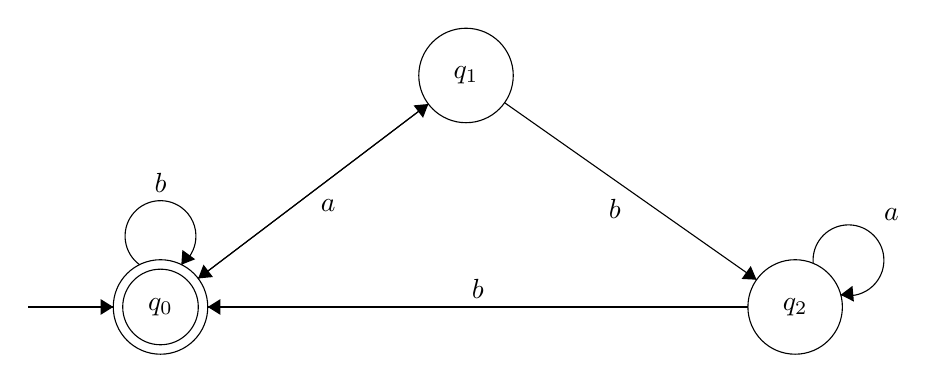
\begin{tikzpicture}[scale=0.2]
\tikzstyle{every node}+=[inner sep=0pt]
\draw [black] (8.6,-18) circle (3);
\draw (8.6,-18) node {$q_0$};
\draw [black] (8.6,-18) circle (2.4);
\draw [black] (28,-3.3) circle (3);
\draw (28,-3.3) node {$q_1$};
\draw [black] (48.9,-18) circle (3);
\draw (48.9,-18) node {$q_2$};
\draw [black] (0.2,-18) -- (5.6,-18);
\fill [black] (5.6,-18) -- (4.8,-17.5) -- (4.8,-18.5);
\draw [black] (7.277,-15.32) arc (234:-54:2.25);
\draw (8.6,-10.75) node [above] {$b$};
\fill [black] (9.92,-15.32) -- (10.8,-14.97) -- (9.99,-14.38);
\draw [black] (45.9,-18) -- (11.6,-18);
\fill [black] (11.6,-18) -- (12.4,-18.5) -- (12.4,-17.5);
\draw (28.75,-17.5) node [above] {$b$};
\draw [black] (50.046,-15.24) arc (185.18593:-102.81407:2.25);
\draw (54.52,-12.1) node [right] {$a$};
\fill [black] (51.79,-17.23) -- (52.63,-17.66) -- (52.54,-16.66);
\draw [black] (30.45,-5.03) -- (46.45,-16.27);
\fill [black] (46.45,-16.27) -- (46.08,-15.4) -- (45.5,-16.22);
\draw (37.45,-11.15) node [below] {$b$};
\draw [black] (10.99,-16.19) -- (25.61,-5.11);
\fill [black] (25.61,-5.11) -- (24.67,-5.2) -- (25.27,-5.99);
\draw (19.25,-11.15) node [below] {$a$};
\draw [black] (25.61,-5.11) -- (10.99,-16.19);
\fill [black] (10.99,-16.19) -- (11.93,-16.1) -- (11.33,-15.31);
\end{tikzpicture}
\end{center}

\vspace{5mm}

\noindent\textbf{Solution:}

\vspace{5mm}

\begin{center}
\begin{tikzpicture}[scale=0.2]
\tikzstyle{every node}+=[inner sep=0pt]
\draw [black] (19.5,-18) circle (3);
\draw (19.5,-18) node {$q_0$};
\draw [black] (38.9,-3.3) circle (3);
\draw (38.9,-3.3) node {$q_1$};
\draw [black] (59.8,-18) circle (3);
\draw (59.8,-18) node {$q_2$};
\draw [black] (7.6,-18) circle (3);
\draw [black] (19.5,-29.8) circle (3);
\draw [black] (19.5,-29.8) circle (2.4);
\draw [black] (18.177,-15.32) arc (234:-54:2.25);
\draw (19.5,-10.75) node [above] {$b$};
\fill [black] (20.82,-15.32) -- (21.7,-14.97) -- (20.89,-14.38);
\draw [black] (56.8,-18) -- (22.5,-18);
\fill [black] (22.5,-18) -- (23.3,-18.5) -- (23.3,-17.5);
\draw (39.65,-17.5) node [above] {$b$};
\draw [black] (60.946,-15.24) arc (185.18593:-102.81407:2.25);
\draw (65.42,-12.1) node [right] {$a$};
\fill [black] (62.69,-17.23) -- (63.53,-17.66) -- (63.44,-16.66);
\draw [black] (41.35,-5.03) -- (57.35,-16.27);
\fill [black] (57.35,-16.27) -- (56.98,-15.4) -- (56.4,-16.22);
\draw (48.35,-11.15) node [below] {$b$};
\draw [black] (21.89,-16.19) -- (36.51,-5.11);
\fill [black] (36.51,-5.11) -- (35.57,-5.2) -- (36.17,-5.99);
\draw (30.15,-11.15) node [below] {$a$};
\draw [black] (36.51,-5.11) -- (21.89,-16.19);
\fill [black] (21.89,-16.19) -- (22.83,-16.1) -- (22.23,-15.31);
\draw [black] (10.6,-18) -- (16.5,-18);
\fill [black] (16.5,-18) -- (15.7,-17.5) -- (15.7,-18.5);
\draw (13.55,-17.5) node [above] {$\epsilon$};
\draw [black] (0.2,-18) -- (4.6,-18);
\fill [black] (4.6,-18) -- (3.8,-17.5) -- (3.8,-18.5);
\draw [black] (19.5,-21) -- (19.5,-26.8);
\fill [black] (19.5,-26.8) -- (20,-26) -- (19,-26);
\draw (19,-23.9) node [left] {$\epsilon$};
\end{tikzpicture}
\end{center}

\noindent First we'll add a dummy starting and accepting state, and now we'll start by removing $q_1$.

\vspace{5mm}

\noindent\includegraphics[width=\textwidth]{first-dfa}

\vspace{5mm}

\noindent After removing $q_1$ we have the following NFA. Now to remove $q_2$.

\vspace{5mm}

\noindent\includegraphics[width=\textwidth]{second-dfa}

\vspace{5mm}

\noindent After removing $q_2$ we have the following NFA. Now to remove $q_0$.

\vspace{5mm}

\noindent\includegraphics[width=\textwidth]{third-dfa}

\vspace{5mm}

\noindent Now all the states have been removed, besides the dummy ones, meaning that we are at our final answer with the corresponding regular expression for the NFA being:

\vspace{5mm}

\LARGE\noindent \textbf{$\epsilon ((b+aa)^*aba^*b)^* \epsilon$}

\end{document}
